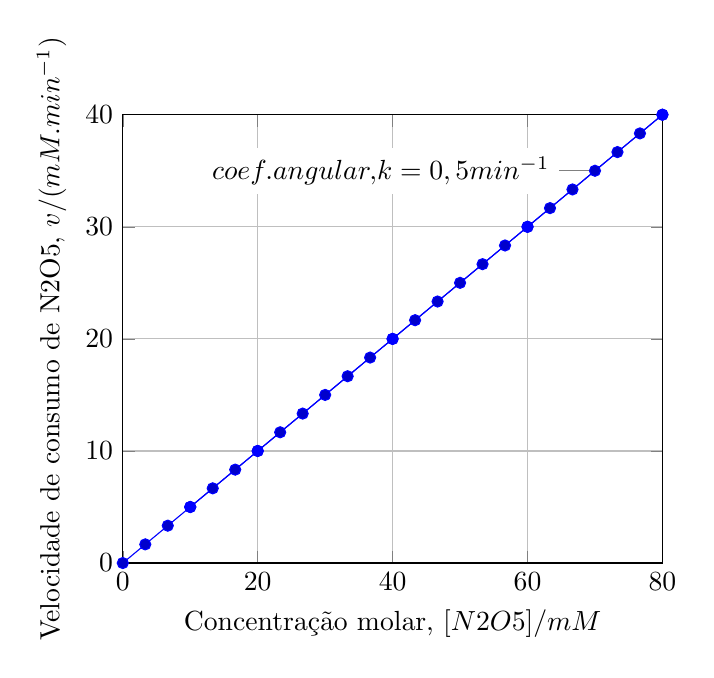
\begin{tikzpicture}
    \begin{axis}
        [
            xlabel = {Concentração molar, $[\ce{N2O5}]/\unit{mM}$},
            ylabel = {Velocidade de consumo de \ce{N2O5}, $v/(\unit{mM.min^{-1}})$},
            xmin = 0, xmax = 80,
            ymin = 0, ymax = 40,
            domain = 0:80,
            grid = major,
        ]

    \addplot+ [blue]
        {
            x/2
        };
        
    \addplot [mark=*, color=blue] coordinates
        { 
            (10,5) 
            (20,10) 
            (40,20) 
            (60,30) 
            (80,40) 
        };
    \node[coordinate,pin={[fill=white] left:{$\text{coef. angular, } k = \qty{0,5}{min^{-1}}$}}] 
        at (axis cs:70,35)   {};

    \end{axis}
\end{tikzpicture}